\section{Software Design Process}
\label{sec:design}

The software design process has been inspired by the \Gls{use_case} 2.0 \cite{jacobson2011usecase} of Iva Jacobsen \textit{et al.}. This approach is an extension of the \gls{UML} definition for \glspl{use_case} and includes a more specific approach how to deal with different layers of abstraction. This helps to guide the requirement analysis in an efficient way and enables easy communication between software engineers and non-coders. A brief overview of the used approach can be found in \autoref{fig:usecase20:flow}.

\begin{figure}[!ht]
\centering
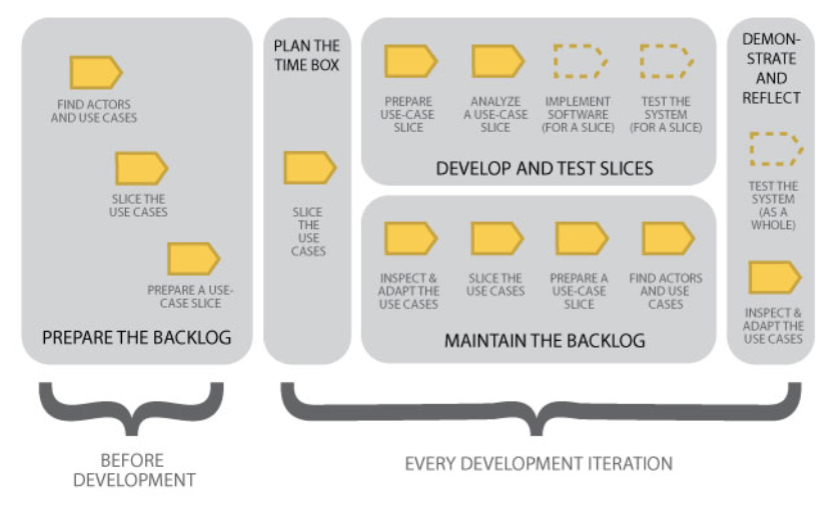
\includegraphics[width=0.8\textwidth]{figures/uc20_flow}
\caption{\gls{use_case} 2.0 activities for iterative development approaches \cite{jacobson2011usecase}}
\label{fig:usecase20:flow}
\end{figure}


\subsection{Use-Cases, Use-Case Flows and Use-Case Slices}
Use cases are the core concept in Use Case 2.0. In addition to the \gls{UML} specification \glspl{use_case} are described as cards including the attributes Priority, Release, Size and Complexity. For the prioritisation the MoSCoW \cite{moscow} (Must, Should, Could, Won't) is used. After the initial requirement analysis, \glspl{use_case_slice} are generated usually including flows, tests and an estimation of the development. In this step the different \glspl{Actor} are identified and test cases are defined. To do so, the \glspl{use_case_slice} are analysed to check how the system elements will interact to perform the assigned \gls{use_case}. The \glspl{use_case_slice} are then going to be implemented and tested with the previous defined test scenarios. Finally the whole system will be tested with \glspl{e2e_test}.

\textbf{\Glspl{use_case}} are the general tasks the system and the actors will perform. They are big, not thought completely through and do not contain directly implementable tasks.

\textbf{\Glspl{use_case_flow}} are the different flows, how the interaction between actors and the system take place. Usually there is a standard flow, and alternative (error / exception handling) flows. These will be specified later when we go deeper into the analysis. In the state of Use Case Flows we will as well generate Test Cases for the flows. 

\textbf{\Glspl{use_case_slice}} are the final development tasks. They will be generated out of the Use Case Flows and can be independently implemented as a single iteration step. They are bases on the Flows and Test Cases. Further Test Cases are usually generated during the implementation react on system specific scenarios.


\subsection{Test Driven development}
\label{sec:tdd}
\Gls{TDD} encourages simple designs and modularity of software products \cite{tdd}. Many companies therefore employ a \gls{TDD} process. The underlying project of this dissertation uses \gls{RoR} which has test driven mechanics build in its core framework (\texttt{rspec}). In combination with the introduced Use Case 2.0 approach, \gls{TDD} can be easily used to ensure correctnes between the specification of a \gls{use_case} and the actual implementation. In general \gls{TDD} is constructed out of following steps which are applied iterative: 

\bigskip

\begin{enumerate}
	\item Adding a test.
	\item Running all test and seeing the recently added test fail.
	\item Implementing the actual feature.
	\item Running the tests again and make them pass.
	\item Refactoring of the written code.
\end{enumerate}

\bigskip

One key component in \gls{TDD} is to keep it short and simple (KISS principle), which results in small, testable and reusable modules in a software and usually leads to better code quality. As the software will be developed in iterative steps, the progress is easily trackable and although changes are made to already existing features, the integrated tests for the previously implemented functionality ensures the continuous integrity of the overall system.  

In our case \glspl{unit_test}, \glspl{integration_test} and \glspl{e2e_test} have been used to test the overall system. As described in \autoref{sub:technical} a \gls{CI} has been setup to ensure this continuous integrity of the system. The implemented \glspl{e2e_test} are basically described by the standard- and alternative-flows that are attached to each \gls{use_case} as defined in \autoref{sub:use_cases}. The individual tests that were executed can be found in \autoref{sub:test_suit} in the appendix.


